\chapter{Contribution}
Spatial filtering is a types of finite impulse response (FIR) filtering. It is a mask of weights with shape as rectangular. It mean that sliding the mask along the image and apply to multiplication and collection operation on the pixels protected by the mask. 

\section*{Original Image }
First, we are going to read and show original image as below :
%\begin{lstlisting}
%I = imread('lena.tif');
%F = imshow(I);
%\end{lstlisting}

%\textbf{Result:}
\begin{center}
	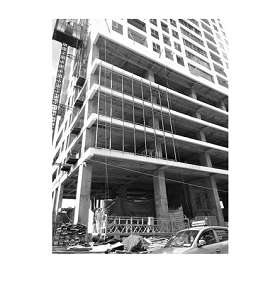
\includegraphics{construction.png}

 Original Image

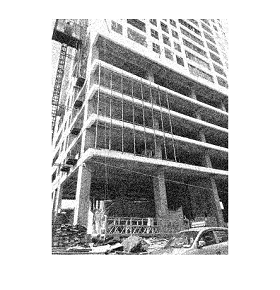
\includegraphics{noisec.png}

Add noise (gaussian noise \& 0.05 variance.)





\end{center}

\section{Median Filter}
Median Filter is family of order filters. It has process : Replace the value of a pixel with the median value of the neighborhood.

$I_{median} = median(I[i,j])$  with $(i,j)\in neighborhood$
\vspace{2cm}
\begin{center}
	

\begin{tabular}{|c|c|c|}  
	\hline 
	30 & 10 & 20 \\ 
	\hline                    
	10 & 250 & 25 \\ 
	\hline 
	20 & 25 & 30 \\ 
	\hline 
\end{tabular} 
\end{center}
\

\



$\Rightarrow$ 10 10 20 20 \textbf{25} 25 30 30 250 

\hspace{26mm}$\uparrow$

\hspace{20mm} median

\newpage
\textbf{Result:}
\vspace{2cm}

\begin{center}
	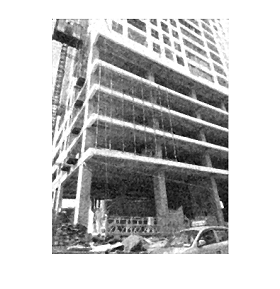
\includegraphics{medianc3.png}
	
	Filter 3$\times$3
\end{center}

\begin{center}
	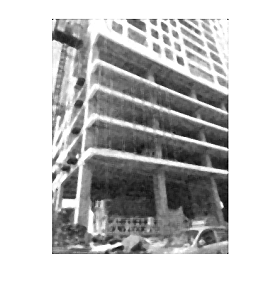
\includegraphics{medianc5.png}

	Filter 5$\times$5
\end{center}
\newpage


\begin{center}
	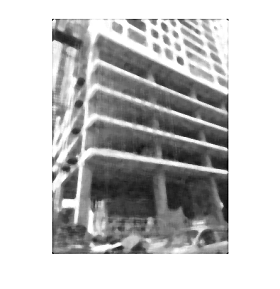
\includegraphics{medianc7.png}
	
		Filter 7$\times$7
\end{center}
\section{Average Filter}

\

Feature: 

Average Filter is spatial filter that applies to a neighborhood (local method). It's a linear filter as a convolution. This mean a pixel is replaced by the average of itself and its neighbours which size determines the amount of smoothing. And equivalent to a filtering operation lowpass.


\

Average Filter have: 
\begin{center}
	Filter 3$\times$3

$\dfrac{1}{9}\begin{tabular}{|c|c|c|}
\hline 
1 & 1 & 1 \\ 
\hline 
1 & 1 & 1 \\ 
\hline 
1 & 1 & 1 \\ 
\hline 
\end{tabular}$ 	
\end{center}

\

\begin{center}
		Filter 5$\times$5
	
	$\dfrac{1}{25}\begin{tabular}{|c|c|c|c|c|}
		\hline 
		1 & 1 & 1 & 1 & 1 \\ 
		\hline 
		1 & 1 & 1 & 1 & 1 \\ 
		\hline 
		1 & 1 & 1 & 1 & 1 \\ 
		\hline 
		1 & 1 & 1 & 1 & 1 \\ 
		\hline 
		1 & 1 & 1 & 1 & 1 \\ 
		\hline 
	\end{tabular} $
\end{center}

\

\begin{center}
	Filter 7$\times$7

$\dfrac{1}{49}\begin{tabular}{|c|c|c|c|c|c|c|}
	\hline 
	1 & 1 & 1 & 1 & 1 & 1 & 1 \\ 
	\hline 
	1 & 1 & 1 & 1 & 1 & 1 & 1 \\ 
	\hline 
	1 & 1 & 1 & 1 & 1 & 1 & 1 \\ 
	\hline 
	1 & 1 & 1 & 1 & 1 & 1 & 1 \\ 
	\hline 
	1 & 1 & 1 & 1 & 1 & 1 & 1 \\ 
	\hline 
	1 & 1 & 1 & 1 & 1 & 1 & 1 \\ 
	\hline 
	1 & 1 & 1 & 1 & 1 & 1 & 1 \\ 
	\hline 
\end{tabular} $
\end{center}
\vspace{1cm}


\textbf{Result:}

\begin{center}
	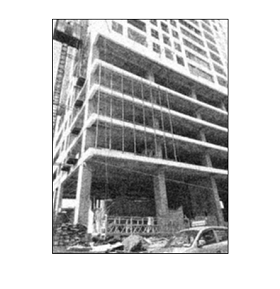
\includegraphics{avec3.png}
	
	Filter $3\times3$
	
	 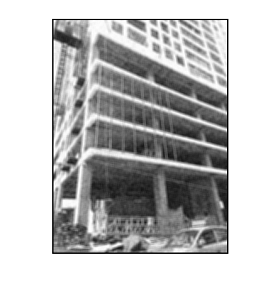
\includegraphics{avec5.png}
	
	Filter $5\times5$
	
		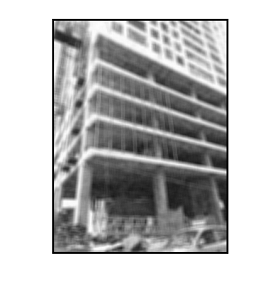
\includegraphics{avec7.png}
	
Filter $7\times7$
\end{center}

\section{Gaussian Filter}

The Gaussian kernel in dimension 2:
\vspace{0.5cm}

$G(x,y) = \dfrac{1}{2\pi\sigma^2}\exp\left[-\dfrac{(x-\mu_x)^2+(y-\mu_y)^2}{2\sigma^2}\right ]$

\vspace{0.5cm}

Define the Gaussian mask($\sigma = 2$):
\vspace{1cm}
%$$\mu = 0$$
%$$
\begin{center}
	Filter 3$\times$3

$\dfrac{1}{16}\begin{tabular}{|c|c|c|}
	\hline 
	1 & 2 & 1 \\ 
	\hline 
	2 & 4 & 2 \\ 
	\hline 
	1 & 2 & 1 \\ 
	\hline 
\end{tabular} $
\end{center}

\begin{center}
	Filter 5$\times$5

$\dfrac{1}{273}\begin{tabular}{|c|c|c|c|c|}
	\hline 
	1 & 4 & 7 & 4 & 1 \\ 
	\hline 
	4 & 16 & 26 & 16 & 4 \\ 
	\hline 
	7 & 26 & 41 & 26 & 7 \\ 
	\hline 
	4 & 16 & 26 & 16 & 4 \\ 
	\hline 
	1 & 4 & 7 & 4 & 1 \\ 
	\hline 
\end{tabular}$ 
\end{center}

\begin{center}
	Filter 7$\times$7

$\dfrac{1}{1003}$\begin{tabular}{|c|c|c|c|c|c|c|}
	\hline 
	0 & 0 & 1 & 2 & 1 & 0 & 0 \\ 
	\hline 
	0 & 3 & 13 & 22 & 13 & 3 & 0 \\ 
	\hline 
	1 & 13 & 59 & 97 & 59 & 13 & 1 \\ 
	\hline 
	2 & 22 & 97 & 159 & 97 & 22 & 2 \\ 
	\hline 
	1 & 13 & 59 & 97 & 59 & 13 & 1 \\ 
	\hline 
	0 & 3 & 13 & 22 & 13 & 3 & 0 \\ 
	\hline 
	0 & 0 & 1 & 2 & 1 & 0 & 0 \\ 
	\hline 
\end{tabular} 
\end{center}
\vspace{1cm}

From theory above, we are going to build function for gaussian filter :
\newpage
\textbf{Result:}

\begin{center}
	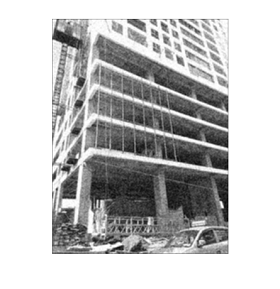
\includegraphics{gauc3.png}
	
	Filter $3\times3$
	
	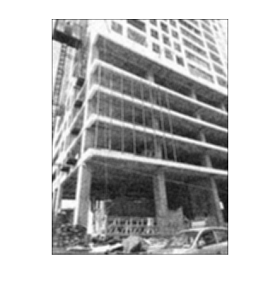
\includegraphics{gauc5.png}
	
	Filter $5\times5$
	
	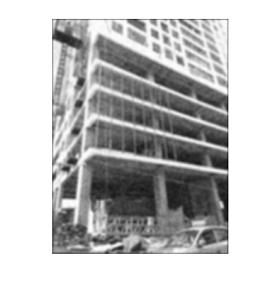
\includegraphics{gauc7.png}
	
	Filter $7\times7$
\end{center}

\section{Wiener Filter}


\textbf{Result:}
\vspace{1cm}
\begin{center}
\includegraphics{Wienec3.png}

Filter $3\times3$

\includegraphics{Wienec5.png}

Filter $5\times5$

\includegraphics{Wienec7.png}

Filter $7\times7$

\end{center}






